\documentclass[journal,12pt,twocolumn]{IEEEtran}
%
\usepackage{setspace}
\usepackage{gensymb}
%\doublespacing
\singlespacing

%\usepackage{graphicx}
%\usepackage{amssymb}
%\usepackage{relsize}
\usepackage[cmex10]{amsmath}
%\usepackage{amsthm}
%\interdisplaylinepenalty=2500
%\savesymbol{iint}
%\usepackage{txfonts}
%\restoresymbol{TXF}{iint}
%\usepackage{wasysym}
\usepackage{amsthm}
%\usepackage{iithtlc}
\usepackage{mathrsfs}
\usepackage{txfonts}
\usepackage{stfloats}
\usepackage{bm}
\usepackage{cite}
\usepackage{cases}
\usepackage{subfig}
%\usepackage{xtab}
\usepackage{longtable}
\usepackage{multirow}
%\usepackage{algorithm}
%\usepackage{algpseudocode}
\usepackage{enumitem}
\usepackage{mathtools}
\usepackage{steinmetz}
\usepackage{tikz}
\usepackage{circuitikz}
\usepackage{verbatim}
\usepackage{tfrupee}
\usepackage[breaklinks=true]{hyperref}
%\usepackage{stmaryrd}
\usepackage{tkz-euclide} % loads  TikZ and tkz-base
%\usetkzobj{all}
\usetikzlibrary{calc,math}
\usepackage{listings}
    \usepackage{color}                                            %%
    \usepackage{array}                                            %%
    \usepackage{longtable}                                        %%
    \usepackage{calc}                                             %%
    \usepackage{multirow}                                         %%
    \usepackage{hhline}                                           %%
    \usepackage{ifthen}                                           %%
  %optionally (for landscape tables embedded in another document): %%
    \usepackage{lscape}     
\usepackage{multicol}
\usepackage{chngcntr}
%\usepackage{enumerate}

%\usepackage{wasysym}
%\newcounter{MYtempeqncnt}
\DeclareMathOperator*{\Res}{Res}
%\renewcommand{\baselinestretch}{2}
\renewcommand\thesection{\arabic{section}}
\renewcommand\thesubsection{\thesection.\arabic{subsection}}
\renewcommand\thesubsubsection{\thesubsection.\arabic{subsubsection}}

\renewcommand\thesectiondis{\arabic{section}}
\renewcommand\thesubsectiondis{\thesectiondis.\arabic{subsection}}
\renewcommand\thesubsubsectiondis{\thesubsectiondis.\arabic{subsubsection}}

% correct bad hyphenation here
\hyphenation{op-tical net-works semi-conduc-tor}
\def\inputGnumericTable{}                                 %%

\lstset{
%language=C,
frame=single, 
breaklines=true,
columns=fullflexible
}
%\lstset{
%language=tex,
%frame=single, 
%breaklines=true
%}

\begin{document}
%


\newtheorem{theorem}{Theorem}[section]
\newtheorem{problem}{Problem}
\newtheorem{proposition}{Proposition}[section]
\newtheorem{lemma}{Lemma}[section]
\newtheorem{corollary}[theorem]{Corollary}
\newtheorem{example}{Example}[section]
\newtheorem{definition}[problem]{Definition}
%\newtheorem{thm}{Theorem}[section] 
%\newtheorem{defn}[thm]{Definition}
%\newtheorem{algorithm}{Algorithm}[section]
%\newtheorem{cor}{Corollary}
\newcommand{\BEQA}{\begin{eqnarray}}
\newcommand{\EEQA}{\end{eqnarray}}
\newcommand{\define}{\stackrel{\triangle}{=}}
\bibliographystyle{IEEEtran}
%\bibliographystyle{ieeetr}
\providecommand{\mbf}{\mathbf}
\providecommand{\pr}[1]{\ensuremath{\Pr\left(#1\right)}}
\providecommand{\qfunc}[1]{\ensuremath{Q\left(#1\right)}}
\providecommand{\sbrak}[1]{\ensuremath{{}\left[#1\right]}}
\providecommand{\lsbrak}[1]{\ensuremath{{}\left[#1\right.}}
\providecommand{\rsbrak}[1]{\ensuremath{{}\left.#1\right]}}
\providecommand{\brak}[1]{\ensuremath{\left(#1\right)}}
\providecommand{\lbrak}[1]{\ensuremath{\left(#1\right.}}
\providecommand{\rbrak}[1]{\ensuremath{\left.#1\right)}}
\providecommand{\cbrak}[1]{\ensuremath{\left\{#1\right\}}}
\providecommand{\lcbrak}[1]{\ensuremath{\left\{#1\right.}}
\providecommand{\rcbrak}[1]{\ensuremath{\left.#1\right\}}}
\theoremstyle{remark}
\newtheorem{rem}{Remark}
\newcommand{\sgn}{\mathop{\mathrm{sgn}}}
\providecommand{\abs}[1]{\left\vert#1\right\vert}
\providecommand{\res}[1]{\Res\displaylimits_{#1}} 
\providecommand{\norm}[1]{\left\lVert#1\right\rVert}
%\providecommand{\norm}[1]{\lVert#1\rVert}
\providecommand{\mtx}[1]{\mathbf{#1}}
\providecommand{\mean}[1]{E\left[ #1 \right]}
\providecommand{\fourier}{\overset{\mathcal{F}}{ \rightleftharpoons}}
%\providecommand{\hilbert}{\overset{\mathcal{H}}{ \rightleftharpoons}}
\providecommand{\system}{\overset{\mathcal{H}}{ \longleftrightarrow}}
	%\newcommand{\solution}[2]{\textbf{Solution:}{#1}}
\newcommand{\solution}{\noindent \textbf{Solution: }}
\newcommand{\cosec}{\,\text{cosec}\,}
\providecommand{\dec}[2]{\ensuremath{\overset{#1}{\underset{#2}{\gtrless}}}}
\newcommand{\myvec}[1]{\ensuremath{\begin{pmatrix}#1\end{pmatrix}}}
\newcommand{\mydet}[1]{\ensuremath{\begin{vmatrix}#1\end{vmatrix}}}
%\numberwithin{equation}{section}
\numberwithin{equation}{subsection}
%\numberwithin{problem}{section}
%\numberwithin{definition}{section}
\makeatletter
\@addtoreset{figure}{problem}
\makeatother
\let\StandardTheFigure\thefigure
\let\vec\mathbf
%\renewcommand{\thefigure}{\theproblem.\arabic{figure}}
%\renewcommand{\thefigure}{\theproblem}
\renewcommand{\thefigure}{\thesection}
\renewcommand{\thetable}{\thesection}
%\setlist[enumerate,1]{before=\renewcommand\theequation{\theenumi.\arabic{equation}}
%\counterwithin{equation}{enumi}
%\renewcommand{\theequation}{\arabic{subsection}.\arabic{equation}}
\def\putbox#1#2#3{\makebox[0in][l]{\makebox[#1][l]{}\raisebox{\baselineskip}[0in][0in]{\raisebox{#2}[0in][0in]{#3}}}}
     \def\rightbox#1{\makebox[0in][r]{#1}}
     \def\centbox#1{\makebox[0in]{#1}}
     \def\topbox#1{\raisebox{-\baselineskip}[0in][0in]{#1}}
     \def\midbox#1{\raisebox{-0.5\baselineskip}[0in][0in]{#1}}
%\vspace{3cm}
\title{Physical Layer Design for a Narrow Band Communication System}
\author{G V V Sharma}
%\title{
%	\logo{Matrix Analysis through Octave}{\begin{center}\includegraphics[scale=.24]{tlc}\end{center}}{}{HAMDSP}
%}
% paper title
% can use linebreaks \\ within to get better formatting as desired
%\title{Matrix Analysis through Octave}
%
%
% author names and IEEE memberships
% note positions of commas and nonbreaking spaces ( ~ ) LaTeX will not break
% a structure at a ~ so this keeps an author's name from being broken across
% two lines.
% use \thanks{} to gain access to the first footnote area
% a separate \thanks must be used for each paragraph as LaTeX2e's \thanks
% was not built to handle multiple paragraphs
%
%\author{<-this % stops a space
%\thanks{}}
%}
% note the % following the last \IEEEmembership and also \thanks - 
% these prevent an unwanted space from occurring between the last author name
% and the end of the author line. i.e., if you had this:
% 
% \author{....lastname \thanks{...} \thanks{...} }
%                     ^------------^------------^----Do not want these spaces!
%
% a space would be appended to the last name and could cause every name on that
% line to be shifted left slightly. This is one of those "LaTeX things". For
% instance, "\textbf{A} \textbf{B}" will typeset as "A B" not "AB". To get
% "AB" then you have to do: "\textbf{A}\textbf{B}"
% \thanks is no different in this regard, so shield the last } of each \thanks
% that ends a line with a % and do not let a space in before the next \thanks.
% Spaces after \IEEEmembership other than the last one are OK (and needed) as
% you are supposed to have spaces between the names. For what it is worth,
% this is a minor point as most people would not even notice if the said evil
% space somehow managed to creep in.
% The paper headers
%\markboth{Journal of \LaTeX\ Class Files,~Vol.~6, No.~1, January~2007}%
%{Shell \MakeLowercase{\textit{et al.}}: Bare Demo of IEEEtran.cls for Journals}
% The only time the second header will appear is for the odd numbered pages
% after the title page when using the twoside option.
% 
% *** Note that you probably will NOT want to include the author's ***
% *** name in the headers of peer review papers.                   ***
% You can use \ifCLASSOPTIONpeerreview for conditional compilation here if
% you desire.
% If you want to put a publisher's ID mark on the page you can do it like
% this:
%\IEEEpubid{0000--0000/00\$00.00~\copyright~2007 IEEE}
% Remember, if you use this you must call \IEEEpubidadjcol in the second
% column for its text to clear the IEEEpubid mark.
% make the title area
\maketitle
\newpage
%\tableofcontents
\bigskip
\renewcommand{\thefigure}{\theenumi}
\renewcommand{\thetable}{\theenumi}
%\renewcommand{\theequation}{\theenumi}
%\begin{abstract}
%%\boldmath
%In this letter, an algorithm for evaluating the exact analytical bit error rate  (BER)  for the piecewise linear (PL) combiner for  multiple relays is presented. Previous results were available only for upto three relays. The algorithm is unique in the sense that  the actual mathematical expressions, that are prohibitively large, need not be explicitly obtained. The diversity gain due to multiple relays is shown through plots of the analytical BER, well supported by simulations. 
%
%\end{abstract}
% IEEEtran.cls defaults to using nonbold math in the Abstract.
% This preserves the distinction between vectors and scalars. However,
% if the journal you are submitting to favors bold math in the abstract,
% then you can use LaTeX's standard command \boldmath at the very start
% of the abstract to achieve this. Many IEEE journals frown on math
% in the abstract anyway.
% Note that keywords are not normally used for peerreview papers.
%\begin{IEEEkeywords}
%Cooperative diversity, decode and forward, piecewise linear
%\end{IEEEkeywords}
% For peer review papers, you can put extra information on the cover
% page as needed:
% \ifCLASSOPTIONpeerreview
% \begin{center} \bfseries EDICS Category: 3-BBND \end{center}
% \fi
%
% For peerreview papers, this IEEEtran command inserts a page break and
% creates the second title. It will be ignored for other modes.
%\IEEEpeerreviewmaketitle
\begin{abstract}
This a simple document explaining a question about the concept of similar triangles.
\end{abstract}
Download all python codes from 
%
\begin{lstlisting}
svn co https://github.com/SiddharthPh/Summer2020/trunk/geometry/codes
\end{lstlisting}
%
and latex-tikz codes from 
%
\begin{lstlisting}
svn co https://github.com/gadepall/school/trunk/ncert/geometry/figs
\end{lstlisting}
%
\section{Specifications}
\begin{enumerate}[label=\thesubsection.\arabic*.,ref=\thesubsection.\theenumi]

\numberwithin{equation}{enumi}
\numberwithin{figure}{enumi}
\item Constellation diagram of BPSK 
\begin{figure}[!h]
		\resizebox{\columnwidth}{!}{
\begin{tikzpicture}

\draw[<->,thick] (-4,0)--(4,0) node[right]{$\phi_1$};
\draw[<->,thick] (0,-4)--(0,4) node[above]{$\phi_2$};

\filldraw[black] (2.5,0) circle (2pt) node[below] {$s_0$} ;
\filldraw[black] (0,2.5) circle (2pt) node[left] {$s_1$} ;
\filldraw[black] (-2.5,0) circle (2pt) node[below] {$s_2$} ;
\filldraw[black] (0,-2.5) circle (2pt) node[left] {$s_3$} ;

\end{tikzpicture}
}
\caption{Constellation diagram}
\label{fig:ee18btech11042_1}
\end{figure}
\item Encoding 
\newline 
We will encode bits as  symbols $s_0$ and $s_1$.Here, we will transmit $s_0$ if bit is 0 and we transmit $s_1$ if bit is 1.


\[ s =   \left\{
\begin{array}{cc}

    s_0 ,&     bit = 0 \\
    s_1, &     bit = 1 \\
\end{array}
\right .\]

 



\item Decision rule for BPSK.
\newline
Given symbols $s_0$ and $ s_1$ are equiprobable and assume symbol carries $\sqrt{E_b}$ per bit and consider a  additive white gaussian noise(AWGN) with mean 0 and variance $\frac{N_o}{2}$ and take  symbols as equiprobable. The received symbols can be:
\begin{align}
    y|s_0 = \sqrt(E_b) + n
    \label{eq:ee18btech11042_1}
\end{align}
\begin{align}
    y|s_1 = -\sqrt(E_b) + n
    \label{eq:ee18btech11042_2}
\end{align}
According to MAP detction rule, we will decode the received signal  as symbol s for which  p\brak{s|y} is more.
\begin{align}
    \hat{s} = max_{s \in  \cbrak{s_0,s_1}} p\brak{s|y}
    \label{eq:ee18btech11042_3}
\end{align}
\begin{align}
    \implies p\brak{s_0|y} \dec{s_0}{s_1} p\brak{s_1|y}
    \label{eq:ee18btech11042_4}
\end{align}
Using Bayes rule,
\begin{align}
    p\brak{s_0|y} = \frac{p\brak{y|s_0}p\brak{s_0}}{p\brak{y}}
    \label{eq:ee18btech11042_5}
\end{align}
\begin{align}
    p\brak{s_1|y} = \frac{p\brak{y|s_1}p\brak{s_1}}{p\brak{y}}
    \label{eq:ee18btech11042_6}
\end{align}
Since symbols are equi probable. p\brak{s_0} \&  p\brak{s_1} are equal.
\begin{align}
    \frac{p\brak{y|s_0}p\brak{s_0}}{p\brak{y}} \dec{s_0}{s_1}  \frac{p\brak{y|s_1}p\brak{s_1}}{p\brak{y}}
    \label{eq:ee18btech11042_7}
\end{align}
\begin{align}
    \implies p\brak{y|s_0} \dec{s_0}{s_1} p\brak{y|s_1}
    \label{eq:ee18btech11042_8}
\end{align}
\begin{align}
    \implies \frac{1}{\sqrt{2\pi}} \exp{-\frac{(y-\sqrt{E_b})^2}{\frac{N_o}{2}}}  \dec{s_0}{s_1}   
\\
    \frac{1}{\sqrt{2\pi}} \exp{-\frac{(y+\sqrt{E_b})^2}{\frac{N_o}{2}}}
    \label{eq:ee18btech11042_9}
\end{align}

\begin{align}
     \implies (y+\sqrt{E_b})^2 \dec{s_0}{s_1} (y - \sqrt{E_b})^2
     \label{eq:ee18btech11042_10}
\end{align}
\begin{align}
    \implies y \dec{s_0}{s_1} 0
    \label{eq:ee18btech11042_11}
\end{align}
The decision region of BPSK is:
\begin{align}
    y \dec{s_0}{s_1} 0
    \label{eq:ee18btech11042_12}
\end{align}
\begin{figure}[!h]
		\resizebox{\columnwidth}{!}{\begin{circuitikz}[american]


    \ctikzset{tripoles/mos style/arrows}
    \draw[<->] (-5,0)--(5,0)node[right]{$x$};
    \draw[-,dashed] (0,-5)--(0,5);
    \filldraw[black](-2.5,0) circle(2pt) node[below] {$s_1$};
    \filldraw[black](2.5,0) circle(2pt) node[below] {$s_0$};
    \filldraw[black](0,0) circle(2pt) node[below] {$o$};
    \coordinate[label = left:$D_1$]  (a) at (4,3);
    \coordinate[label = left:$D_2$]  (a) at (-4,3 );
    \end{circuitikz}
}
\caption{Decision region for BPSK}
\label{fig:ee18btech11042_2}
\end{figure}
\item Decoding 
\newline
Consider, y is the received symbol .Then, we need to decode this symbol into bits.Here,we will  use decision region  to decode into bits.
\[ bit =   \left\{
\begin{array}{cc}

    y>0 ,&     bit = 0 \\
    y<0, &     bit = 1 \\
\end{array}
\right .\]
So, if received symbol y $>$0 ,we decode that symbol into 0  and if y$<$0 we decode it as 1.
\item The following code has simulation of ber of BPSK.
\begin{lstlisting}
 codes/bpsk_ber.py
\end{lstlisting}


\end{enumerate}



%In right triangle ABC, right angled at C, M is
%the mid-point of hypotenuse AB. C is joined to
%M and produced to a point D such that DM =
%CM. Point D is joined to point B. Show that
%
%\begin{enumerate}[label = (\alph*)]
%\item $\triangle  AMC  \cong   \triangle  BMD $
%\item $\triangle DBC $ is a right angle.
%\item $\triangle  DBC  \cong  \triangle  ABC $
%\item $CM = \frac{1}{2} AB$
%\end{enumerate}
%\section{Construction}
%\renewcommand{\theequation}{\theenumi}
\begin{enumerate}[label=\thesection.\arabic*.,ref=\thesection.\theenumi]
\numberwithin{equation}{enumi}
\item The figure for A triangle obtained in the question looks like Fig. \ref{fig:tri_right_angle}.
with angles $\phase{ A},\phase{ C}$ and $\phase{ B}$ and sides $a, b$ and $c$.  The unique feature of this triangle is $\phase{ C}$ which is defined to be $90\degree$.


%\renewcommand{\thefigure}{\theenumi.\arabic{figure}}
\begin{figure}[!ht]
\centering
\resizebox{\columnwidth}{!}{

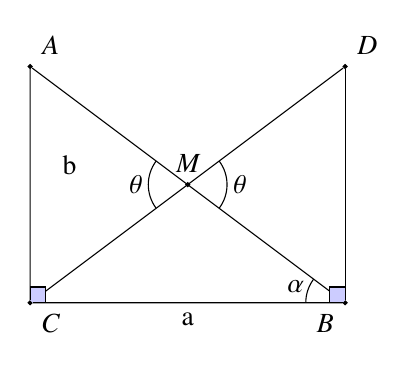
\begin{tikzpicture}
[scale=1,>=stealth,point/.style={draw,circle,fill = black,inner sep=0.5pt},]

%Triangle sides
\def\a{4}
\def\b{3}
\def\c{sqrt(\a^2+\c^2)}



%Labeling points
\node (A) at (0,\b)[point,label=above right:$A$] {};
\node (B) at (\a, 0)[point,label=below left:$B$] {};
\node (C) at (0, 0)[point,label=below right:$C$] {};
\node (M) at (\a*0.5,\b*0.5)[point,label=above:$M$] {};
\node (D) at (\a,\b)[point,label=above right:$D$] {};


%Drawing triangle ABC
\draw (A) -- node[left] {$\textrm{}$} (B) -- node[below] {$\textrm{a}$} (C) -- node[above,xshift=5mm] {$\textrm{b}$} (A);

%Joining CD
\draw (C)--(D);
%Joining BD
\draw (B)--(D);

%Drawing and marking angles
\tkzMarkAngle[fill=orange!40,size=0.5cm,mark=](A,M,C)
\tkzMarkAngle[fill=orange!40,size=0.5cm,mark=](B,M,D)
\tkzMarkAngle[fill=green!40,size=0.5cm,mark=](A,B,C)
\tkzMarkRightAngle[fill=blue!20,size=.2](A,C,B)
\tkzMarkRightAngle[fill=blue!20,size=.2](D,B,C)
\tkzLabelAngle[pos=0.65](A,M,C){$\theta$}
\tkzLabelAngle[pos=0.65](B,M,D){$\theta$}
\tkzLabelAngle[pos=0.65](A,B,C){$\alpha$}


\end{tikzpicture}
}
\caption{Right Angled Triangle by Latex-Tikz}
\label{fig:tri_right_angle}	
\end{figure}
%
%
%\renewcommand{\thefigure}{\theenumi}
%
\item List the design parameters for construction
\label{const:table1}
\\
\solution See Table. \ref{table:table1}. 
%
\begin{table}[ht!]
\centering
%\begin{tabular}{ |p{3cm}|p{3cm}|  }
%\hline
% \multicolumn{2}{|c|}{Initial Input Values.} \\
%\hline
%a & 4\\
%\hline
%b & 3\\
%\hline
%$\phase{(ACB)$ & $90^{\circ}$ \\
%\hline
%\end{tabular}
%%%%%%%%%%%%%%%%%%%%%%%%%%%%%%%%%%%%%%%%%%%%%%%%%%%%%%%%%%%%%%%%%%%%%%
%%                                                                  %%
%%  This is the header of a LaTeX2e file exported from Gnumeric.    %%
%%                                                                  %%
%%  This file can be compiled as it stands or included in another   %%
%%  LaTeX document. The table is based on the longtable package so  %%
%%  the longtable options (headers, footers...) can be set in the   %%
%%  preamble section below (see PRAMBLE).                           %%
%%                                                                  %%
%%  To include the file in another, the following two lines must be %%
%%  in the including file:                                          %%
%%        \def\inputGnumericTable{}                                 %%
%%  at the beginning of the file and:                               %%
%%        \input{name-of-this-file.tex}                             %%
%%  where the table is to be placed. Note also that the including   %%
%%  file must use the following packages for the table to be        %%
%%  rendered correctly:                                             %%
%%    \usepackage[latin1]{inputenc}                                 %%
%%    \usepackage{color}                                            %%
%%    \usepackage{array}                                            %%
%%    \usepackage{longtable}                                        %%
%%    \usepackage{calc}                                             %%
%%    \usepackage{multirow}                                         %%
%%    \usepackage{hhline}                                           %%
%%    \usepackage{ifthen}                                           %%
%%  optionally (for landscape tables embedded in another document): %%
%%    \usepackage{lscape}                                           %%
%%                                                                  %%
%%%%%%%%%%%%%%%%%%%%%%%%%%%%%%%%%%%%%%%%%%%%%%%%%%%%%%%%%%%%%%%%%%%%%%



%%  This section checks if we are begin input into another file or  %%
%%  the file will be compiled alone. First use a macro taken from   %%
%%  the TeXbook ex 7.7 (suggestion of Han-Wen Nienhuys).            %%
\def\ifundefined#1{\expandafter\ifx\csname#1\endcsname\relax}


%%  Check for the \def token for inputed files. If it is not        %%
%%  defined, the file will be processed as a standalone and the     %%
%%  preamble will be used.                                          %%
\ifundefined{inputGnumericTable}

%%  We must be able to close or not the document at the end.        %%
	\def\gnumericTableEnd{\end{document}}


%%%%%%%%%%%%%%%%%%%%%%%%%%%%%%%%%%%%%%%%%%%%%%%%%%%%%%%%%%%%%%%%%%%%%%
%%                                                                  %%
%%  This is the PREAMBLE. Change these values to get the right      %%
%%  paper size and other niceties.                                  %%
%%                                                                  %%
%%%%%%%%%%%%%%%%%%%%%%%%%%%%%%%%%%%%%%%%%%%%%%%%%%%%%%%%%%%%%%%%%%%%%%

	\documentclass[12pt%
			  %,landscape%
                    ]{report}
       \usepackage[latin1]{inputenc}
       \usepackage{fullpage}
       \usepackage{color}
       \usepackage{array}
       \usepackage{longtable}
       \usepackage{calc}
       \usepackage{multirow}
       \usepackage{hhline}
       \usepackage{ifthen}

	\begin{document}


%%  End of the preamble for the standalone. The next section is for %%
%%  documents which are included into other LaTeX2e files.          %%
\else

%%  We are not a stand alone document. For a regular table, we will %%
%%  have no preamble and only define the closing to mean nothing.   %%
    \def\gnumericTableEnd{}

%%  If we want landscape mode in an embedded document, comment out  %%
%%  the line above and uncomment the two below. The table will      %%
%%  begin on a new page and run in landscape mode.                  %%
%       \def\gnumericTableEnd{\end{landscape}}
%       \begin{landscape}


%%  End of the else clause for this file being \input.              %%
\fi

%%%%%%%%%%%%%%%%%%%%%%%%%%%%%%%%%%%%%%%%%%%%%%%%%%%%%%%%%%%%%%%%%%%%%%
%%                                                                  %%
%%  The rest is the gnumeric table, except for the closing          %%
%%  statement. Changes below will alter the table's appearance.     %%
%%                                                                  %%
%%%%%%%%%%%%%%%%%%%%%%%%%%%%%%%%%%%%%%%%%%%%%%%%%%%%%%%%%%%%%%%%%%%%%%

\providecommand{\gnumericmathit}[1]{#1} 
%%  Uncomment the next line if you would like your numbers to be in %%
%%  italics if they are italizised in the gnumeric table.           %%
%\renewcommand{\gnumericmathit}[1]{\mathit{#1}}
\providecommand{\gnumericPB}[1]%
{\let\gnumericTemp=\\#1\let\\=\gnumericTemp\hspace{0pt}}
 \ifundefined{gnumericTableWidthDefined}
        \newlength{\gnumericTableWidth}
        \newlength{\gnumericTableWidthComplete}
        \newlength{\gnumericMultiRowLength}
        \global\def\gnumericTableWidthDefined{}
 \fi
%% The following setting protects this code from babel shorthands.  %%
 \ifthenelse{\isundefined{\languageshorthands}}{}{\languageshorthands{english}}
%%  The default table format retains the relative column widths of  %%
%%  gnumeric. They can easily be changed to c, r or l. In that case %%
%%  you may want to comment out the next line and uncomment the one %%
%%  thereafter                                                      %%
\providecommand\gnumbox{\makebox[0pt]}
%%\providecommand\gnumbox[1][]{\makebox}

%% to adjust positions in multirow situations                       %%
\setlength{\bigstrutjot}{\jot}
\setlength{\extrarowheight}{\doublerulesep}

%%  The \setlongtables command keeps column widths the same across  %%
%%  pages. Simply comment out next line for varying column widths.  %%
\setlongtables

\setlength\gnumericTableWidth{%
	56pt+%
	33pt+%
0pt}
\def\gumericNumCols{2}
\setlength\gnumericTableWidthComplete{\gnumericTableWidth+%
         \tabcolsep*\gumericNumCols*2+\arrayrulewidth*\gumericNumCols}
\ifthenelse{\lengthtest{\gnumericTableWidthComplete > \linewidth}}%
         {\def\gnumericScale{\ratio{\linewidth-%
                        \tabcolsep*\gumericNumCols*2-%
                        \arrayrulewidth*\gumericNumCols}%
{\gnumericTableWidth}}}%
{\def\gnumericScale{1}}

%%%%%%%%%%%%%%%%%%%%%%%%%%%%%%%%%%%%%%%%%%%%%%%%%%%%%%%%%%%%%%%%%%%%%%
%%                                                                  %%
%% The following are the widths of the various columns. We are      %%
%% defining them here because then they are easier to change.       %%
%% Depending on the cell formats we may use them more than once.    %%
%%                                                                  %%
%%%%%%%%%%%%%%%%%%%%%%%%%%%%%%%%%%%%%%%%%%%%%%%%%%%%%%%%%%%%%%%%%%%%%%

\ifthenelse{\isundefined{\gnumericColA}}{\newlength{\gnumericColA}}{}\settowidth{\gnumericColA}{\begin{tabular}{@{}p{56pt*\gnumericScale}@{}}x\end{tabular}}
\ifthenelse{\isundefined{\gnumericColB}}{\newlength{\gnumericColB}}{}\settowidth{\gnumericColB}{\begin{tabular}{@{}p{33pt*\gnumericScale}@{}}x\end{tabular}}

\begin{tabular}[c]{%
	b{\gnumericColA}%
	b{\gnumericColB}%
	}

%%%%%%%%%%%%%%%%%%%%%%%%%%%%%%%%%%%%%%%%%%%%%%%%%%%%%%%%%%%%%%%%%%%%%%
%%  The longtable options. (Caption, headers... see Goosens, p.124) %%
%	\caption{The Table Caption.}             \\	%
% \hline	% Across the top of the table.
%%  The rest of these options are table rows which are placed on    %%
%%  the first, last or every page. Use \multicolumn if you want.    %%

%%  Header for the first page.                                      %%
%	\multicolumn{2}{c}{The First Header} \\ \hline 
%	\multicolumn{1}{c}{colTag}	%Column 1
%	&\multicolumn{1}{c}{colTag}	\\ \hline %Last column
%	\endfirsthead

%%  The running header definition.                                  %%
%	\hline
%	\multicolumn{2}{l}{\ldots\small\slshape continued} \\ \hline
%	\multicolumn{1}{c}{colTag}	%Column 1
%	&\multicolumn{1}{c}{colTag}	\\ \hline %Last column
%	\endhead

%%  The running footer definition.                                  %%
%	\hline
%	\multicolumn{2}{r}{\small\slshape continued\ldots} \\
%	\endfoot

%%  The ending footer definition.                                   %%
%	\multicolumn{2}{c}{That's all folks} \\ \hline 
%	\endlastfoot
%%%%%%%%%%%%%%%%%%%%%%%%%%%%%%%%%%%%%%%%%%%%%%%%%%%%%%%%%%%%%%%%%%%%%%

\hhline{|-|-}
	 \multicolumn{1}{|p{\gnumericColA}|}%
	{\gnumericPB{\centering}\gnumbox{Parameter}}
	&\multicolumn{1}{p{\gnumericColB}|}%
	{\gnumericPB{\centering}\gnumbox{Value}}
\\
\hhline{|--|}
	 \multicolumn{1}{|p{\gnumericColA}|}%
	{\gnumericPB{\centering}\gnumbox{$a$}}
	&\multicolumn{1}{p{\gnumericColB}|}%
	{\gnumericPB{\centering}\gnumbox{4}}
\\
\hhline{|--|}
	 \multicolumn{1}{|p{\gnumericColA}|}%
	{\gnumericPB{\centering}\gnumbox{$b$}}
	&\multicolumn{1}{p{\gnumericColB}|}%
	{\gnumericPB{\centering}\gnumbox{3}}
\\
\hhline{|--|}
	 \multicolumn{1}{|p{\gnumericColA}|}%
	{\gnumericPB{\centering}\gnumbox{$\phase{ACB}$}}
	&\multicolumn{1}{p{\gnumericColB}|}%
	{\gnumericPB{\centering}\gnumbox{90\degree}}
\\
\hhline{|-|-|}
\end{tabular}

\ifthenelse{\isundefined{\languageshorthands}}{}{\languageshorthands{\languagename}}
\gnumericTableEnd

\caption{To construct $\triangle ACB$}
\label{table:table1}	
\end{table}

%\item
%	For simplicity, let the greek letter $\alpha = \phase{ B$.  We have the following definitions.
%\begin{equation}
%\label{eq:tri_trig_defs}
%\begin{matrix}
	%\sin \theta = \frac{b}{c} & 	\cos \theta = \frac{a}{c} \\
	%\tan \theta = \frac{c}{a} & \cot \theta = \frac{1}{\tan \theta} \\
	%\csc \theta = \frac{1}{\sin \theta} & \sec \theta = \frac{1}{\cos \theta}
	%\end{equation}
%
\item Find the coordinates of the various points in Fig. \ref{fig:tri_right_angle}
\label{const:tri_right_angle}
\\
%
\solution From the given information, 
%$\triangle ABC$ are 
\begin{align}
\label{eq:constr_a}
\vec{A} &= \myvec{0\\b} 
\\
 \vec{C} &= \myvec{0\\0}, 
\label{eq:constr_c}
\\
\vec{B} &= \myvec{a\\0}
\label{eq:constr_b}
\end{align}
$\because \vec{M}$ is the midpoint of $AB$,
\begin{align}
\vec{M}= \frac{\vec{A}+\vec{B}}{2} = \frac{1}{2}\myvec{a\\b}
\label{eq:constr_m}
\end{align}
%
Also, $\vec{M}$ is given to be the midpoint of $C$.  Hence, 
\begin{align}
\vec{M}&= \frac{\vec{C}+\vec{D}}{2}
\\
\implies \vec{D} &= 2 \vec{M} - \vec{C} = \myvec{a\\b}
\label{eq:constr_d}
\end{align}
%
The values are listed in 
%\item List the  derived values.
%\label{const:table2}
%\\
%\solution See  
Table. \ref{table:table2} 
\begin{table}[ht!]
\centering
\begin{tabular}{ |p{3cm}|p{3cm}|  }
\hline
 \multicolumn{2}{|c|}{Derived Values.} \\
\hline
$\vec{M}$ & $$\begin{pmatrix}2\\1.5\end{pmatrix}$$\\						
\hline
$\vec{D}$ & $$\begin{pmatrix}4\\3\end{pmatrix} $$\\
\hline
\end{tabular}
\caption{To construct $\triangle DCB$}
\label{table:table2}
\end{table}
%
\item Draw Fig. \ref{fig:tri_right_angle}.	
\\
\solution The  following Python code generates Fig. \ref{fig:tri_sss_py}
%
\begin{lstlisting}
codes/triangle.py
\end{lstlisting}
\begin{figure}[!ht]
\centering
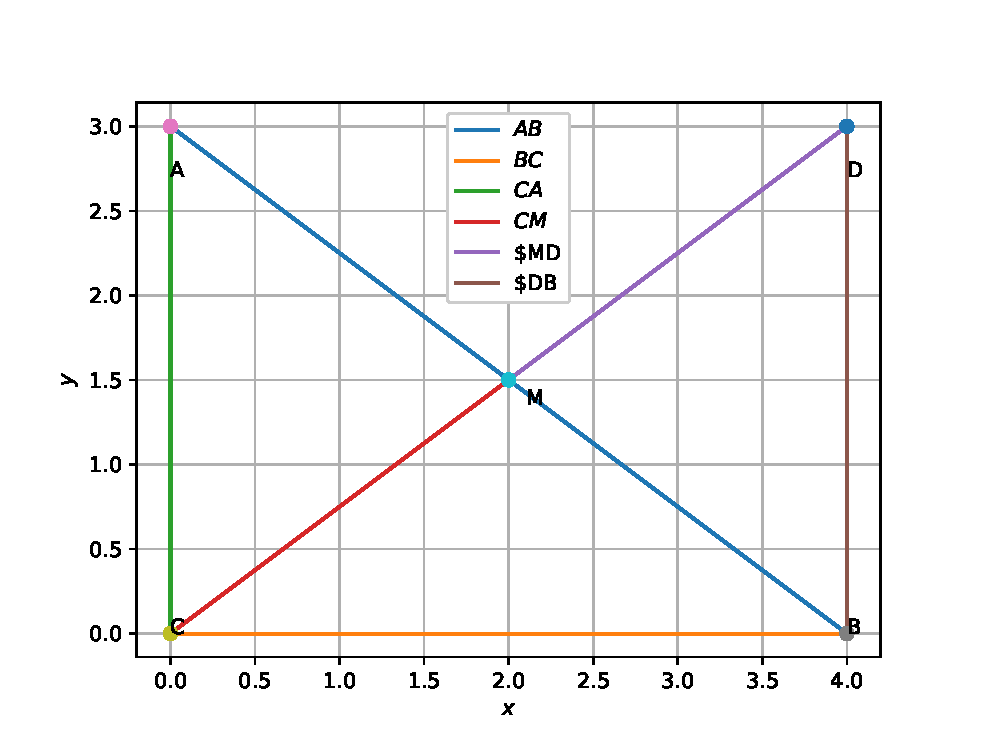
\includegraphics[width=\columnwidth]{./figs/triangle.eps}
\caption{Triangle generated using python}
\label{fig:tri_sss_py}
\end{figure}

%
and the equivalent latex-tikz code generating Fig. \ref{fig:tri_right_angle} is 
\begin{lstlisting}
figs/triangle.tex
\end{lstlisting}
%
The above latex code can be compiled as a standalone document as
\begin{lstlisting}
figs/triangle_fig.tex
\end{lstlisting}

%

%

%
%

\end{enumerate}


%
%
%\section{Solution}
%\renewcommand{\theequation}{\theenumi}
\begin{enumerate}[label=\thesection.\arabic*.,ref=\thesection.\theenumi]
\numberwithin{equation}{enumi}
	
\item $\triangle AMC \cong \triangle DMB$  by SAS congruency $\because$
\begin{enumerate}
\item $AM = BM$
\item $CM = DM$
\item $\phase{AMC}$ = $\phase{DMB}$ ( Vertically Opposite Angles)
\end{enumerate}
%
\item From \eqref{eq:constr_b}, \eqref{eq:constr_c} and \eqref{eq:constr_d},
%
%
\begin{align}
\brak{\vec{D}-\vec{B}}^T
\brak{\vec{B}-\vec{C}} &= \myvec{0 & b}\myvec{a \\ 0} = 0
\\
\implies BD \perp BC
\end{align}
%
\item From \eqref{eq:constr_a}, \eqref{eq:constr_b}, \eqref{eq:constr_c} and \eqref{eq:constr_d},
\begin{align}
\norm{\vec{A}-\vec{B}} &= \norm{\myvec{-a \\ b}}
\\
\norm{\vec{C}-\vec{D}} &= \norm{\myvec{-a \\ -b}}
\\
\implies \norm{\vec{A}-\vec{B}} &= \norm{\vec{C}-\vec{D}}\\
\text{or, } AB &=CD
\label{eq:solution_abcd}
\end{align}
%
From RHS congruence,  $\triangle ACB \cong  \triangle DCB$.
\item From \eqref{eq:solution_abcd}, noting that $\vec{M}$ is the mid point of both $AB$ and $CD$, 
\begin{align}
CM = \frac{1}{2}CD =\frac{1}{2} AB
\end{align}



\end{enumerate}

%\subsection{Sol.a)}
%\input{./chapters/sol_a.tex}
%\subsection{Sol.b)}
%\input{./chapters/sol_b.tex}
%\subsection{Sol.c)}
%\input{./chapters/sol_c.tex}
%\subsection{Sol.d)}
%Since $\vec{CM}$ is halfway of $\vec{CD}$
\newline
$\norm{\vec{CM}}=\norm{\vec{CD}}$
\newline
From Solution b) it is clear that $\norm{\vec{CD}}=\norm{\vec{BA}}$
\newline
Therefore $\norm{\vec{CM}}=\frac{1}{2}\norm{\vec{AB}}$
\\
Hence, proved.

\end{document}









